Planetary positions influence on psychology

Vedic astrology, also known as Jyotish, is an ancient system of astrology that originated in the Indian subcontinent. It is considered one of the oldest astrological systems in the world and has its roots in the Vedas, the ancient sacred texts of Hinduism.
Vedic astrology is one of the most important limb(Vedanga) out of the total six limbs(Vedangas) found in the ancient Indian scriptures. The origins of Vedic astrology can be traced back to around 1500 BCE, during the late Vedic period. It is classified into the three major branches or disciplines known as the Siddhanta, Samhita and Hora. These branches provide different approaches and methods for studying and practicing astrology.
\begin{itemize}
	\item \textbf{Siddhanta:} Siddhanta deals with all the mathematical calculations of space \& time which is involed in the study of planets, stars, comets and contellations present in the space. It is also referred as the Astronomy in modern days.
	\item \textbf{Samhita:} Samhita, also known as Muhurtha, is the branch of Vedic astrology that deals with collective or mundane astrology. It focuses on predicting and analyzing events and phenomena on a broader scale, such as natural disasters, weather patterns, political developments, and societal events.
	\item \textbf{Hora:} Hora or horarian astrology is the branch of Vedic astrology that specifically deals with individual horoscopes or birth charts (Jataka).
\end{itemize}

\begin{sanskrit}
	\begin{center}
		अथ खेटा रविश्चन्द्रो मङ्गलश्च बुधस्तथा।\\गुरुः शुक्रः शनि राहुः केतुश्चैते यथाक्रमम्‌॥३:११॥\cite{BrihatParasharHoraShastraVol1}\cite{wiki:bphs}\label{s1}
		मेषो वृषश्च मिथुनः कर्कसिंहकुमारिकाः।\\तुलालिऽश्च धनुर्नक्रे कुम्भो मीनस्ततः परम्‌॥४:३॥\cite{BrihatParasharHoraShastraVol1}\cite{wiki:bphs}\label{s2}
	\end{center}
\end{sanskrit}
Sun, Moon, Mars, Mercury, Jupiter, Venus, Saturn, Rahu, and Ketu, these are mentioned in order, one by one.\ref{s1}
Aries, Taurus, Gemini, Cancer, Leo, Virgo, Libra, Scorpio, Sagittarius and Pisces are the twelve contellations also known as the zodiac signs.\ref{s2}
However, the main source of all these things are the four basic elements which are the Fire, Water, Wind, Earth \& Sky.

\subsubsection{Significance of Houses}

\subsubsection{Properties of Zodiac Signs}
However, describing all the shlokas here is not possible but properties of the twelve zodiac signs are described in shloka number 7 to 23 of BPHS\cite{BrihatParasharHoraShastraVol1}\cite{wiki:bphs} which are interpreted by the astrologers as follows:
Aries, Taurus, Gemini, Cancer, Leo, Virgo, Libra, Scorpio, Sagittarius and Pisces.

\subsubsection{Properties of Planets}
\begin{sanskrit}
	\begin{center}
		सर्वात्मा च दीवानाथो मनः कुमुदबान्धवः।\\सत्त्वं कुजो बुधैः प्रोक्तो बुधो वाणीप्रदायकः॥३:१३॥\cite{BrihatParasharHoraShastraVol1}\cite{wiki:bphs}
	\end{center}
\end{sanskrit}
\begin{sanskrit}
	\begin{center}
		देवेज्यो ज्ञानसुखदो भृगुर्वीर्यप्रदयकः।\\ऋषिभिः प्राक्‌तनैः प्रोक्तश्छायासूनुश्च दुःखदः॥३:१४॥\cite{BrihatParasharHoraShastraVol1}\cite{wiki:bphs}
	\end{center}
\end{sanskrit}
Jupiter(Brihaspati) is the significator of wisdom. 
Venus(Shukra) is resposible for joy \& ecstacy.
\begin{sanskrit}
	\begin{center}
		रविचन्द्रौ तु राजानौ नेता ज्ञेयो धरात्मजः।\\बुधो राजकुमारश्च सचिवौ गुरुभार्गवौ॥३:१५॥\cite{BrihatParasharHoraShastraVol1}\cite{wiki:bphs}
	\end{center}
\end{sanskrit}
Mars(Mangal) is responsible for the strength of a native which leads to the emotion of anger.
Rahu
\subsubsection{Combinations of Planets with Zodiac Signs}
Effect of different combinations of planets along with the zodiac signs on psychology of human emotions.
However, instead of considering the zodiac signs, one can consider the 27 nakshatras for detailed calculations but for simplicity, we are considering the zodiacs here.
\subsubsection{Dashas \& Transits}
\begin{sanskrit}
	\begin{center}
		विकलानाम् कला षष्ट्या तत्षष्ट्या भाग उच्यते।\\तत्त्रिम्शता भवेद् राशिर् भगणो द्वादशैव ते॥१:२८॥\cite{SuryaSiddhanta}\cite{wiki:ss}
	\end{center}
\end{sanskrit}
60 Vikalas make one kala and 60 kalas make one degree(\textdegree) or one amsa. 30\textdegree(degrees or amsa) make one rashi(one zodiac sign) and twelve such rashies(zodiac signs) make one revolution(bhagana) of the zodiac.

\begin{table}[H]
	\begin{tabular}{|c|c|c|}
		\hline
		\textbf{Graha} & \textbf{Angular Speed} & \textbf{Time For One} \\
		\textbf{(Planet)} & \textbf{(\textdegree/Day)} & \textbf{Zodiac Sign}\\
		\hline
		Surya(Sun) & 1 & 1 Month \\
		\hline
		Chandra(Moon) & 13 & 2.25 Days \\
		\hline
		Brihaspati(Jupiter) & 1/12 & 1 Year \\
		\hline
		Shani(Saturn) & 1/30 & 2.5 Years \\
		\hline
		Budh(Mercury) & 1 & 1 Month \\
		\hline
		Shukra(Venus) & 1 & 1 Month \\
		\hline
		Mangal(Mars) & 2/3 & 1.5 Month \\
		\hline
		Rahu & -1/18 & 18 Months \\
		\hline
		Ketu & -1/18 & 18 Months \\
		\hline
	\end{tabular}
	\caption{Time required by all planets to complete one zodiac sign}
	\label{Table:table}
\end{table}

Table \ref{Table:table} represents the time required by all nine planets to complete one zodiac sign which is calculated in chapter 1, verse 29 to 34 of Surya Siddhanta\cite{SuryaSiddhanta}\cite{wiki:ss}.

Effect of dashaas of the different planets in Chapter number 53 of BPHS.

The planetary vibrations reflected or refracted along with solar radiations to the earth are of varying intensities as per planetary distance, size, and movement in the solar system. These vibrations impact our sensory nerves, mental attitudes, and moods. Thus, it’s very likely that these planetary vibrations supply the energies to the body cells though our nerves. Since these vibrations differ in wavelength intensity and frequency as per the planetary properties and motion; these vibrations supply different sensory stimuli which impacts the human unconscious and personality at the time of birth\cite{article}.
\subsubsection{Sudarshan Chakra}
\begin{sanskrit}
	\begin{center}
		जन्मतो मृत्युपर्यन्तं वर्षमासदिनोद्भवम्।\\शुभं वाऽप्यशुभं सर्वं तच्छृणुष्वैकमानसः॥७४:४॥\cite{BrihatParasharHoraShastraVol2}\cite{wiki:bphs}
	\end{center}
\end{sanskrit}
Physical Level
Mental Level
Spiritual Level
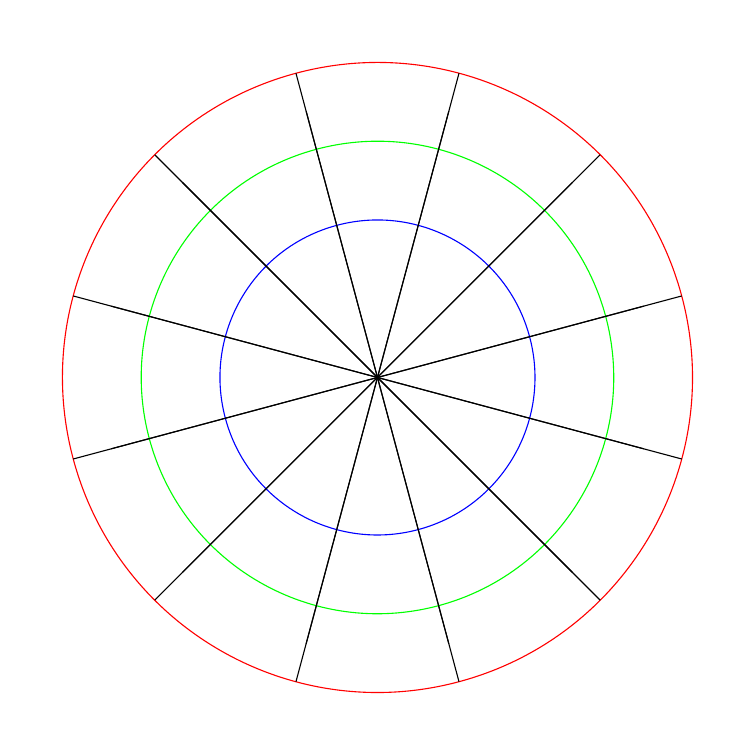
\begin{tikzpicture}[rotate=15]
	\definecolor{mycolor1}{RGB}{255,0,0}
	\definecolor{mycolor2}{RGB}{0,255,0}
	\definecolor{mycolor3}{RGB}{0,0,255}
	\draw[mycolor1] (0,0) circle (4cm);
	\draw[mycolor2] (0,0) circle (3cm);
	\draw[mycolor3] (0,0) circle (2cm);
	\foreach \i in {0,30,...,330}
	{
		\draw (\i:3.5cm) -- (\i+180:4cm);
	}
\end{tikzpicture}